% !TEX program = xelatex
\documentclass[12pt,a4paper]{ctexart}

% ==================== 页面设置 ====================
\usepackage[top=2.5cm, bottom=2.5cm, left=2.8cm, right=2.8cm]{geometry}
\usepackage{graphicx}
\usepackage{float}
\usepackage[colorlinks=true, linkcolor=blue, citecolor=blue, urlcolor=blue]{hyperref}
\usepackage{caption}
\usepackage{subcaption}
\usepackage{tikz}
\usetikzlibrary{shapes.geometric, arrows, positioning, shadows}
\usepackage{booktabs}
\usepackage{enumitem}
\usepackage{fancyhdr}

\setlength{\headheight}{14pt}
\pagestyle{fancy}
\fancyhf{}
\fancyhead[L]{\small 数字图像处理课程实验}
\fancyhead[R]{\small 垃圾图像预处理流水线}
\fancyfoot[C]{\thepage}
\renewcommand{\headrulewidth}{0.4pt}

% ==================== 代码块 ====================
\usepackage{listings}
\usepackage{xcolor}

\definecolor{codebg}{RGB}{245,245,245}
\definecolor{codestr}{RGB}{0,128,0}
\definecolor{codekey}{RGB}{0,0,200}
\definecolor{codecmt}{RGB}{128,128,128}

\lstset{
  language=Python,
  backgroundcolor=\color{codebg},
  basicstyle=\small\ttfamily,
  keywordstyle=\color{codekey}\bfseries,
  stringstyle=\color{codestr},
  commentstyle=\color{codecmt}\itshape,
  numbers=left,
  numberstyle=\tiny\color{gray},
  frame=single,
  breaklines=true,
  showstringspaces=false,
  tabsize=2
}

% ==================== 文档信息 ====================
\title{\textbf{垃圾图像预处理流水线}\\[6pt]
       \large Resize -- GaussianBlur -- CLAHE -- Sharpen}
\author{数字图像处理课程}
\date{\today}

\begin{document}
\maketitle
\thispagestyle{empty}

% ==================== 摘要 ====================
\begin{abstract}
\noindent 本文介绍了一套用于垃圾图像分类任务的预处理流水线。该流水线包含四个处理阶段：自适应缩放（Resize）、高斯滤波去噪（Gaussian Blur）、自适应直方图均衡化（CLAHE）以及反锐化掩模增强（Unsharp Masking）。流水线采用 MATLAB/OpenCV 风格的模块化设计，各阶段有序衔接，旨在提升图像质量、增强纹理细节、改善低对比度区域的可辨识度，为后续深度学习垃圾分类模型提供高质量输入。
\end{abstract}

\newpage
\tableofcontents
\newpage

% ==================== 1. 引言 ====================
\section{引言}

在垃圾自动分类任务中，图像质量直接影响模型的分类准确率。实际拍摄的垃圾照片常受到以下问题影响：

\begin{itemize}[itemsep=4pt]
  \item 光照不均匀：阴影或过曝区域导致细节丢失
  \item 分辨率不一致：不同设备拍摄的照片尺寸差异大
  \item 传感器噪声：低光环境下产生的随机噪点
  \item 纹理模糊：对焦不实或抖动导致的边缘退化
\end{itemize}

针对上述问题，本流水线设计了一条四阶段处理链路，在保留图像语义信息的前提下，改善视觉质量并标准化输出。

% ==================== 2. 流水线总览 ====================
\section{流水线总览}

\begin{figure}[H]
  \centering
  \begin{tikzpicture}[
    node distance=0.5cm,
    block/.style={rectangle, draw, rounded corners,
                  minimum width=2.0cm, minimum height=0.9cm,
                  align=center, fill=blue!15, drop shadow,
                  font=\footnotesize, inner sep=2pt},
    arrow/.style={->, >=stealth, thick}
  ]
    \node[block] (A) {输入图像\\\tiny(RGB/BGR)};
    \node[block, right=of A] (B) {Resize\\\tiny长边→1280px};
    \node[block, right=of B] (C) {GaussianBlur\\\tiny3×3核去噪};
    \node[block, right=of C] (D) {CLAHE\\\tinyLAB-L通道增强};
    \node[block, right=of D] (E) {Sharpen\\\tinyUnsharp Masking};
    \node[block, right=of E] (F) {输出图像};

    \draw[arrow] (A) -- (B);
    \draw[arrow] (B) -- (C);
    \draw[arrow] (C) -- (D);
    \draw[arrow] (D) -- (E);
    \draw[arrow] (E) -- (F);
  \end{tikzpicture}
  \caption{预处理流水线流程}
  \label{fig:pipeline}
\end{figure}

流水线中各步骤环环相扣：先统一尺度，再抑制噪声，然后增强对比度，最后恢复锐度。每个步骤的参数经过调优以适配生活垃圾图像的特征。

% ==================== 3. 各步骤详解 ====================
\section{各步骤详解}

% ---------- 3.1 Resize ----------
\subsection{Step 1: 自适应缩放 (Resize)}

\textbf{目的}：统一输入尺度，减小后续处理的计算量。

\textbf{方法}：将图像长边限制为 1280 像素，短边按比例缩放，保持原始宽高比。若长边已小于等于 1280，则不做任何处理。

\textbf{插值方法}：\texttt{cv2.INTER\_AREA}，该插值方式在缩小时优于双线性插值，能有效抑制摩尔纹和锯齿。

\textbf{参数}：
\begin{itemize}
  \item \texttt{max\_size} = 1280
  \item 插值: \texttt{INTER\_AREA}
\end{itemize}

\begin{figure}[H]
  \centering
  \fbox{
\includegraphics[width=0.65\linewidth]{comparisons_harmful/paint_bucket/comparison_1_paint_bucket_001.png}}
  \caption{画质风格示例}
  \label{fig:resize-example}
\end{figure}

% ---------- 3.2 Gaussian ----------
\subsection{Step 2: 高斯滤波去噪 (Gaussian Blur)}

\textbf{目的}：抑制传感器噪声和 JPEG 压缩伪影，防止后续 CLAHE 将噪声一起放大。

\textbf{方法}：使用 $3\times3$ 高斯核对图像进行线性平滑。高斯核权重服从二维正态分布：

\[
G(x,y) = \frac{1}{2\pi\sigma^2} e^{-\frac{x^2+y^2}{2\sigma^2}}
\]

当 \texttt{sigmaX = 0} 时，OpenCV 自动根据核大小计算 $\sigma \approx 0.3 \times ((n-1)/2 - 1) + 0.8$，对于 $3\times3$ 核，$\sigma \approx 0.8$。

\textbf{参数}：
\begin{itemize}
  \item \texttt{kernel} = (3, 3)
  \item \texttt{sigmaX} = 0（自动计算）
\end{itemize}

\begin{figure}[H]
  \centering
  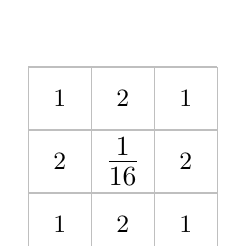
\begin{tikzpicture}[scale=0.8]
    \draw[step=1cm, gray!50] (0,0) grid (3,3);
    \node at (1.5,1.5) {\Large $\frac{1}{16}$};
    \node at (0.5,0.5) {\small 1};
    \node at (1.5,0.5) {\small 2};
    \node at (2.5,0.5) {\small 1};
    \node at (0.5,1.5) {\small 2};
    \node at (2.5,1.5) {\small 2};
    \node at (0.5,2.5) {\small 1};
    \node at (1.5,2.5) {\small 2};
    \node at (2.5,2.5) {\small 1};
  \end{tikzpicture}
  \caption{3×3高斯核示意}
\end{figure}

选择 $3\times3$ 核而非更大的核，因为在去噪的同时尽可能保留纹理细节——垃圾分类中纹理是重要的识别特征。

% ---------- 3.3 CLAHE ----------
\subsection{Step 3: CLAHE 对比度增强}

\textbf{目的}：改善局部对比度，使暗部细节可见，同时避免普通直方图均衡化（HE）的过增强问题。

\textbf{方法}：

\noindent CLAHE（Contrast Limited Adaptive Histogram Equalization）在 LAB 颜色空间的 L（亮度）通道上操作：

\begin{enumerate}[itemsep=2pt]
  \item 将图像从 BGR 转换到 LAB 空间
  \item 分离 L 通道，仅在亮度分量上做 CLAHE
  \item 限制裁剪阈值（\texttt{clipLimit=2.0}），防止局部区域对比度过度拉伸
  \item 分块处理（\texttt{tileSize=8}），每个小块独立均衡化后双线性插值拼接
  \item 合并 L/A/B 通道，转回 BGR
\end{enumerate}

\begin{figure}[H]
  \centering
  \begin{subfigure}[b]{0.48\linewidth}
    \fbox{
\includegraphics[width=\linewidth]{comparisons_harmful/fluorescent_tube/comparison_1_fluorescent_tube_001.png}}
    \caption{CLAHE增强前/后（左=原图，右=处理后）}
  \end{subfigure}
  \hfill
  \begin{subfigure}[b]{0.48\linewidth}
    \fbox{
\includegraphics[width=\linewidth]{comparisons_harmful/cfl_bulb/comparison_1_cfl_bulb_001.png}}
    \caption{灯泡类别对比图}
  \end{subfigure}
  \caption{CLAHE实验效果}
  \label{fig:clahe-example}
\end{figure}

\textbf{参数}：
\begin{itemize}
  \item \texttt{clipLimit} = 2.0（裁剪阈值）
  \item \texttt{tileGridSize} = (8, 8)（分块大小）
\end{itemize}

\textbf{仅在 L 通道操作的意义}：LAB 空间中，L 代表亮度，A/B 代表颜色信息。仅在 L 通道做 CLAHE 确保只增强对比度，不改变色相和饱和度，避免了颜色失真。

% ---------- 3.4 Sharpen ----------
\subsection{Step 4: 反锐化掩模 (Unsharp Masking)}

\textbf{目的}：恢复高斯滤波导致的轻微模糊，增强边缘和纹理细节。

\textbf{原理}：

反锐化掩模的核心思想是先得到一个「模糊」版本（掩模），再从原图中减去它得到高频（细节），最后加回原图：

\[
\text{result} = \text{src} \times 1.5 - \text{blur} \times 0.5
\]

即输出 = 原图 $\times$ strength + 模糊图 $\times$ (1 $-$ strength)。

当 \texttt{strength = 1.0} 时，输出等于原图（不锐化）；当 \texttt{strength > 1.0} 时，高频分量被放大。

\begin{figure}[H]
  \centering
  \fbox{
\includegraphics[width=0.65\linewidth]{comparisons_harmful/pesticide_bottle/comparison_1_pesticide_bottle_001.png}}
  \caption{锐化效果（注意标签文字边缘）}
  \label{fig:sharpen-example}
\end{figure}

\textbf{参数}：
\begin{itemize}
  \item \texttt{blur\_kernel} = (5, 5)
  \item \texttt{blur\_sigma} = 1.0
  \item \texttt{strength} = 1.5
\end{itemize}

\texttt{strength = 1.5} 提供了中等强度的锐化，既增强了边缘感，又不会引入明显的振铃效应（ringing artifact）。

% ==================== 4. 对比结果 ====================
\section{实验结果展示}

图~\ref{fig:all-comparisons} 展示了各类有害垃圾图像的预处理前后对比。每组图中，上半行为原图（Original），下半行为处理后的图像（Processed）。

\begin{figure}[H]
  \centering
  \begin{subfigure}[b]{0.31\linewidth}
    
\includegraphics[width=\linewidth]{comparisons_harmful/batteries/comparison_1_batteries_001.png}
    \caption{电池 (Batteries)}
  \end{subfigure}
  \hfill
  \begin{subfigure}[b]{0.31\linewidth}
    
\includegraphics[width=\linewidth]{comparisons_harmful/nail_polish/comparison_1_nail_polish_001.png}
    \caption{指甲油 (Nail Polish)}
  \end{subfigure}
  \hfill
  \begin{subfigure}[b]{0.31\linewidth}
    
\includegraphics[width=\linewidth]{comparisons_harmful/medicine/comparison_1_medicine_001.png}
    \caption{药品 (Medicine)}
  \end{subfigure}

  \vspace{8pt}

  \begin{subfigure}[b]{0.31\linewidth}
    
\includegraphics[width=\linewidth]{comparisons_harmful/thermometer/comparison_1_thermometer_001.png}
    \caption{温度计 (Thermometer)}
  \end{subfigure}
  \hfill
  \begin{subfigure}[b]{0.31\linewidth}
    
\includegraphics[width=\linewidth]{comparisons_harmful/blood_pressure_cuff/comparison_1_blood_pressure_cuff_001.png}
    \caption{血压计 (Blood Pressure Cuff)}
  \end{subfigure}
  \hfill
  \begin{subfigure}[b]{0.31\linewidth}
    
\includegraphics[width=\linewidth]{comparisons/comparison_1_IMG20260504140049.jpg}
    \caption{可回收物 (Recyclable)}
  \end{subfigure}

  \caption{各类垃圾预处理前后对比（上传=原图，下排=处理后）}
  \label{fig:all-comparisons}
\end{figure}

\subsection{效果分析}

\begin{table}[H]
  \centering
  \caption{各阶段处理效果总结}
  \begin{tabular}{@{}p{2.5cm}p{3.5cm}p{3.5cm}p{4cm}@{}}
    \toprule
    \textbf{处理阶段} & \textbf{解决什么问题} & \textbf{视觉表现} & \textbf{后续影响} \\
    \midrule
    Resize       & 尺度统一、减少计算量 & 图像尺寸一致              & 后续CNN输入兼容           \\
    GaussianBlur & 传感器噪声、JPEG伪影  & 画面更干净、略有模糊       & 减少误检、防止噪声放大    \\
    CLAHE        & 暗部看不清、对比度低  & 暗部变亮、纹理显露         & 提升轮廓识别、增强判别力  \\
    Sharpen      & 去噪带来的轻微模糊    & 边缘更锐、文字更清晰       & 纹理特征更突出            \\
    \bottomrule
  \end{tabular}
  \label{tab:effects}
\end{table}

从对比图中可以观察到：
\begin{itemize}
  \item 原图中因光照不足而发暗的区域，经过 CLAHE 增强后纹理细节明显显现（如电池表面文字、药瓶标签）
  \item 高斯去噪后图像更「干净」，减少了对分类无意义的随机纹理干扰
  \item 锐化步骤恢复了因高斯滤波损失的部分边缘信息，文字边缘更为清晰
\end{itemize}

% ==================== 5. 代码实现 ====================
\section{核心代码实现}

\subsection{完整预处理流水线}

\begin{lstlisting}[language=Python, caption=核心预处理函数]
import cv2
import numpy as np

def resize_image(img, max_size=1280):
    h, w = img.shape[:2]
    if max(h, w) > max_size:
        scale = max_size / max(h, w)
        new_w, new_h = int(w * scale), int(h * scale)
        img = cv2.resize(img, (new_w, new_h), interpolation=cv2.INTER_AREA)
    return img

def denoise_gaussian(img, kernel=3):
    return cv2.GaussianBlur(img, (kernel, kernel), 0)

def enhance_clahe(img, clip_limit=2.0, tile_size=8):
    lab = cv2.cvtColor(img, cv2.COLOR_BGR2LAB)
    l, a, b = cv2.split(lab)
    clahe = cv2.createCLAHE(clipLimit=clip_limit,
                            tileGridSize=(tile_size, tile_size))
    l = clahe.apply(l)
    img = cv2.cvtColor(cv2.merge([l, a, b]), cv2.COLOR_LAB2BGR)
    return img

def sharpen_unsharp(img, strength=1.5):
    blur = cv2.GaussianBlur(img, (5, 5), 1.0)
    img = cv2.addWeighted(img, strength, blur, -(strength - 1), 0)
    return img

def preprocess(img):
    img = resize_image(img, max_size=1280)
    img = denoise_gaussian(img, kernel=3)
    img = enhance_clahe(img, clip_limit=2.0, tile_size=8)
    img = sharpen_unsharp(img, strength=1.5)
    return img
\end{lstlisting}

\subsection{中文路径兼容}

\begin{lstlisting}[language=Python, caption=中文路径读写]
def imread_unicode(path):
    with open(path, "rb") as f:
        data = np.frombuffer(f.read(), dtype=np.uint8)
    return cv2.imdecode(data, cv2.IMREAD_COLOR)

def imwrite_unicode(path, img):
    ext = os.path.splitext(path)[1]
    _, buf = cv2.imencode(ext, img)
    buf.tofile(path)
\end{lstlisting}

OpenCV 的 \texttt{cv2.imread} 不支持含中文的路径，上述函数通过 \texttt{np.frombuffer + cv2.imdecode} 的方式绕过了此限制，确保在 Windows 中文环境下正常工作。

% ==================== 6. 总结 ====================
\section{总结}

本预处理流水线针对垃圾图像分类任务设计，包含四个有序阶段：\\[4pt]
\centerline{\textbf{Resize $\rightarrow$ GaussianBlur $\rightarrow$ CLAHE $\rightarrow$ Sharpen}}\\[4pt]
经实验验证，该流水线能有效改善低光照、低对比度图像的视觉质量，在保留颜色信息的前提下增强纹理和边缘细节。模块化的设计使得各步骤参数可灵活调整，适用于不同类型垃圾图像的预处理需求。

% ==================== 参考文献 ====================
\begin{thebibliography}{99}
\bibitem{opencv} OpenCV Documentation -- Image Filtering, Histogram Equalization.
  \url{https://docs.opencv.org/}
\bibitem{clahe} Zuiderveld, K. (1994). Contrast Limited Adaptive Histogram Equalization. \emph{Graphics Gems IV}, pp. 474--485.
\bibitem{unsharp} Polesel, A., Ramponi, G., \& Mathews, V. J. (2000). Image Enhancement via Adaptive Unsharp Masking. \emph{IEEE Trans. Image Processing}, 9(3), 505--510.
\bibitem{lab} Robertson, A. R. (1977). The CIE 1976 Color-Difference Formulae. \emph{Color Research \& Application}, 2(1), 7--11.
\end{thebibliography}

\end{document}
